% \documentclass[aspectratio=169,notes]{beamer}
\documentclass[aspectratio=169]{beamer}
\usetheme[faculty=phil]{fibeamer}
\usepackage{polyglossia}
\setmainlanguage{english} %% main locale instead of `english`, you
%% can typeset the presentation in either Czech or Slovak,
%% respectively.
\setotherlanguages{russian} %% The additional keys allow
%%
%%   \begin{otherlanguage}{czech}   ... \end{otherlanguage}
%%   \begin{otherlanguage}{slovak}  ... \end{otherlanguage}
%%
%% These macros specify information about the presentation
\title[AGLA1]{Analytical Geometry and Linear Algebra I, Lab 9} %% that will be typeset on the
\subtitle{Conic sections (2nd order curve equation):
\\ a) Parabola  \\ b) Ellipse    
         } %% title page.
\author{Oleg Bulichev}
%% These additional packages are used within the document:
\usepackage{ragged2e}  % `\justifying` text
\usepackage{booktabs}  % Tables
\usepackage{tabularx}
\usepackage{tikz}      % Diagrams
\usetikzlibrary{calc, shapes, backgrounds}
\usepackage{amsmath, amssymb}
\usepackage{url}       % `\url`s
\usepackage{listings}  % Code listings
% \usepackage{subfigure}
\usepackage{floatrow}
\usepackage{subcaption}
\usepackage{mathtools}
\usepackage{todonotes}
\usepackage{fontspec}
\usepackage{multicol}
\usepackage{pdfpages}
\usepackage{wrapfig}
\usepackage{animate}
\usepackage{booktabs}
\usepackage{multirow}

\graphicspath{{resources/}}
\frenchspacing

\setbeamertemplate{caption}[numbered]
\usetikzlibrary{graphs}

% \usepackage[backend=biber,style=ieee,autocite=footnote]{biblatex}
% \addbibresource{biblio.bib}
% \DefineBibliographyStrings{english}{%
%   bibliography = {References},}

\newcommand{\oleg}[2][] {\todo[color=red, #1] {OLEG:\\ #2}}
\newcommand{\fbckg}[1]{\usebackgroundtemplate{\includegraphics[width=\paperwidth]{#1}}}%frame background

\usepackage[framemethod=TikZ]{mdframed}
\newcommand{\dbox}[1]{
\begin{mdframed}[roundcorner=3pt, backgroundcolor=yellow, linewidth=0]
\vspace{1mm}
{#1}
\vspace{1mm}
\end{mdframed}
}

\newcommand{\shf}{\text{shift}}

\begin{document}
\setlength{\abovedisplayskip}{0pt}
\setlength{\belowdisplayskip}{0pt}
\setlength{\abovedisplayshortskip}{0pt}
\setlength{\belowdisplayshortskip}{0pt}

\fbckg{fibeamer/figs/title_page.png}
\frame[c]{\setcounter{framenumber}{0}
    \usebeamerfont{title}%
    \usebeamercolor[fg]{title}%
    \begin{minipage}[b][6.5\baselineskip][b]{\textwidth}%
        \textcolor{black}{\raggedright\inserttitle}
    \end{minipage}
    % \vskip-1.5\baselineskip

    \usebeamerfont{subtitle}%
    \usebeamercolor[fg]{framesubtitle}%
    \begin{minipage}[b][3\baselineskip][b]{\textwidth}
        \raggedright%
        \insertsubtitle%
    \end{minipage}
    \vskip.25\baselineskip
}
%   \frame[c]{\maketitle}
\note{
    \begin{enumerate}
        \item Держать в голове, то что у них потом будет более сложная тема, где есть B.
        \item Сказать им что вначале мы просто тренируемся пользоваться читшитом, а вот на следующей паре будем уже решать реальные задачи
        \item Объяснить general алгоритм для задач: 1) General -> canonical (так как мы только в каноникал знаем формулы) 2) Используя читшит все решаем
        \item Цель изучения коников по мнению Иванова - расширение нейронов. Так же подготовка к изучению advance тем как сложные поверхности итп
        \item Поиск тангента к кривым. Используем формулы без шифта, а потом берез 2 координаты на прямой и сдвигаем их с помощью шифта. Находим новую прямую. Так проще, чем формулу выражать.
    \end{enumerate}
}

\fbckg{fibeamer/figs/common.png}


\begin{frame}[c]{Questions from the class}
    \framesubtitle{}
    \centering
    \textit{ \Large No questions for today}
\end{frame}

\begin{frame}[t]{Questions for today}
    \framesubtitle{}
    \begin{itemize}
        \item How can I work with general form of 2nd order curve equation?
        \item How it relates with cone?
        \item What forms of equation do we have?
    \end{itemize}
\end{frame}

\begin{frame}[t]{Why it is called <<Conic Sections>>}
\framesubtitle{}
    \begin{columns}[T,onlytextwidth]
        \begin{column}{0.69\textwidth}
            The greatest progress in the study of conics by the ancient Greeks is due to \textit{Apollonius of Perga} (died c. 190 BCE), whose eight-volume \textbf{Conic Sections or Conics}. More info \href{https://en.wikipedia.org/wiki/Conic_section}{here}.
            \begin{figure}[H]
                \centering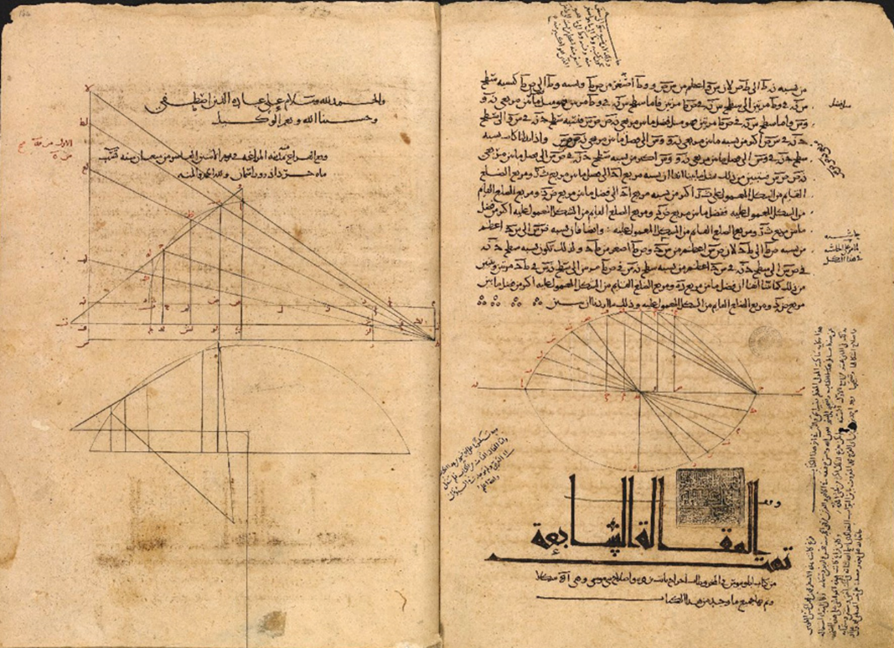
\includegraphics[height=3.5cm,width=1\textwidth,keepaspectratio]{conica_book.png}
                \caption*{Books 5-7 are only available in an Arabic translation (9th century)}
                \label{fig:conica_book.png}
            \end{figure}
        \end{column}
        \begin{column}{0.29\textwidth}
            \vspace{-0.5cm}
            \begin{figure}[H]
                \centering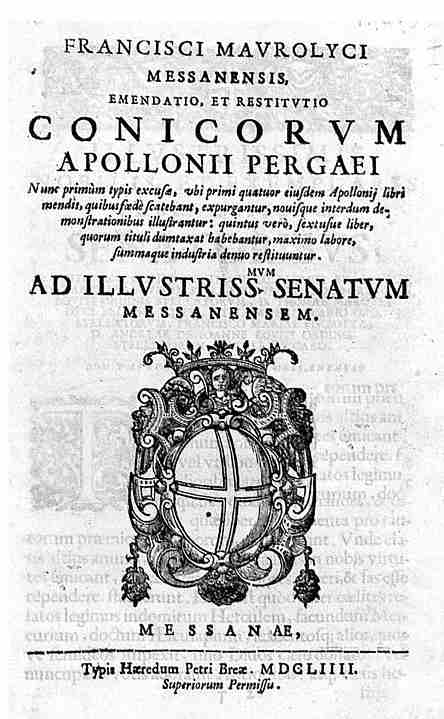
\includegraphics[height=5cm,width=1\textwidth,keepaspectratio]{apollonius_book.jpg}
                \caption*{1654 edition of Conica}
                \label{fig:apollonius_book.jpg}
            \end{figure}
        \end{column}
    \end{columns}
\end{frame}

\begin{frame}[t]{Elliptic Cone}
\framesubtitle{}
    \vspace{-0.6cm}
    \begin{figure}[H]
        \centering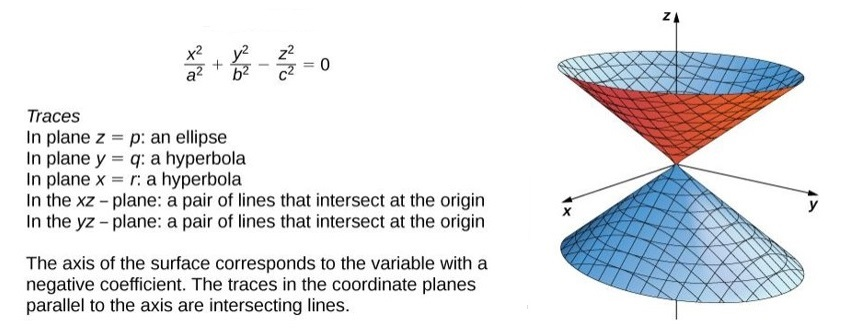
\includegraphics[height=6cm,width=1\textwidth,keepaspectratio]{elliptic_cone.jpg}
        \label{fig:elliptic_cone.jpg}
    \end{figure}
\end{frame}

\begin{frame}[t]{Some definitions, which can be helpful}
\framesubtitle{Eccentricity, Directrix}
    \begin{columns}[T,onlytextwidth]
        \begin{column}{0.59\textwidth}
            \textbf{Eccentricity} is a measure of how much a conic section deviates from being circular. \medskip
        
            It is a constant ration between distance from focal to point on the curve and from the point on the curve to \textbf{directrix}.
        \end{column}
        \begin{column}{0.39\textwidth}
            \vspace{-1cm}
            \begin{figure}[H]
                    \centering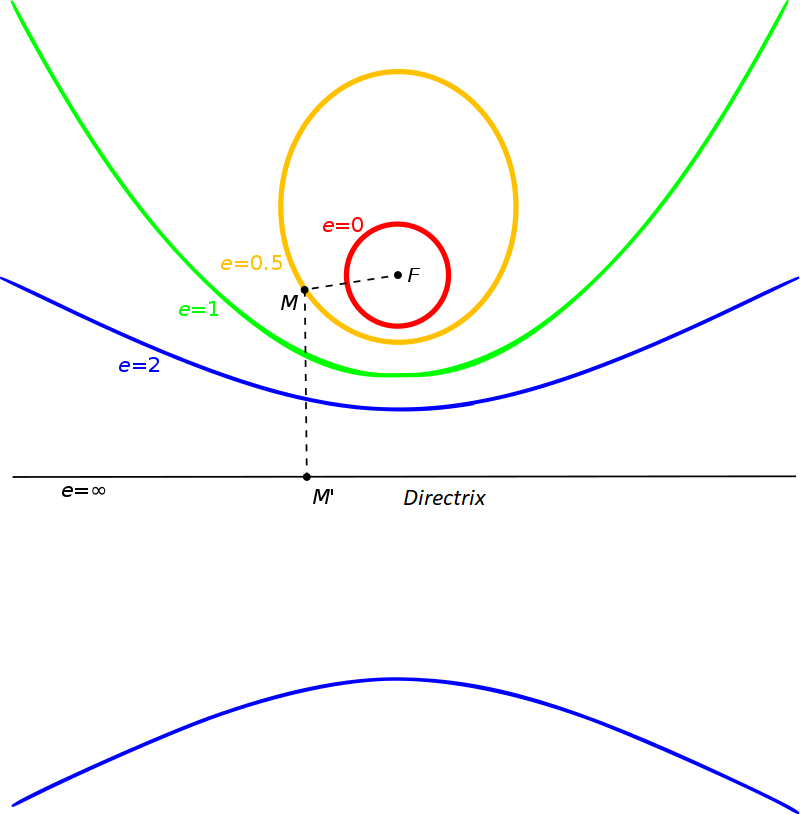
\includegraphics[height=7cm,width=1\textwidth,keepaspectratio]{eccentricity.png}
                    % \caption{capture1}
                    \label{fig:eccentricity.png}
            \end{figure}
        \end{column}
    \end{columns}
\end{frame}

\begin{frame}[t]{Some definitions, which can be helpful}
\framesubtitle{Linear eccentricity, Latus Rectrum, Focal parameter}
    \begin{columns}[T,onlytextwidth]
        \begin{column}{0.59\textwidth}
            The \textbf{linear eccentricity} is the distance between the center and the focus (or one of the two foci). \medskip 
            
            The \textbf{latus rectum} is the chord parallel to the directrix and passing through the focus (or one of the two foci). \medskip 
            
            The \textbf{focal parameter} is the distance from the focus (or one of the two foci) to the directrix.

        \end{column}
        \begin{column}{0.39\textwidth}
            \vspace{-1cm}
            \begin{figure}[H]
                \begin{subfigure}{0.99\textwidth}
                    \centering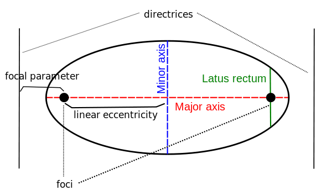
\includegraphics[height=4cm,width=1\textwidth,keepaspectratio]{ellipse_focal.png}
                    % \caption{capture1}
                    \label{fig:ellipse_focal.png}
                \end{subfigure}

                \begin{subfigure}{0.99\textwidth}
                    \vspace{-0.6cm}
                    \centering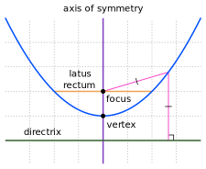
\includegraphics[height=3cm,width=1\textwidth,keepaspectratio]{parabola_focus.png}
                    % \caption{capture2}
                    \label{fig:parabola_focus.png}
                \end{subfigure}
            % \caption{capture_main}
            % \label{fig:}
            \end{figure}
        \end{column}
    \end{columns}
\end{frame}


\begin{frame}[t]{Parabola}
\framesubtitle{}
    \scriptsize
    \vspace{-0.4cm}
\begin{columns}[T,onlytextwidth]
    \begin{column}{0.59\textwidth}
        \textit{Forms:} \\
\begin{itemize}
    \item \textbf{Canonical} $(x-x_{\shf})^2=p(y-y_{\shf})$
    \item \textbf{General} $Ax^2+Bxy+Cy^2+Dx+Ey+F=0$, where either $A=0$ or $C=0$, not both, if $B=0$
    \item \textbf{Parametric} $\left\{\begin{matrix*}[l] x = \sqrt{2}pt\\ y = pt^2\end{matrix*}\right.$
\end{itemize}
    \end{column}
    \begin{column}{0.39\textwidth}
        \begin{figure}[H]
            \centering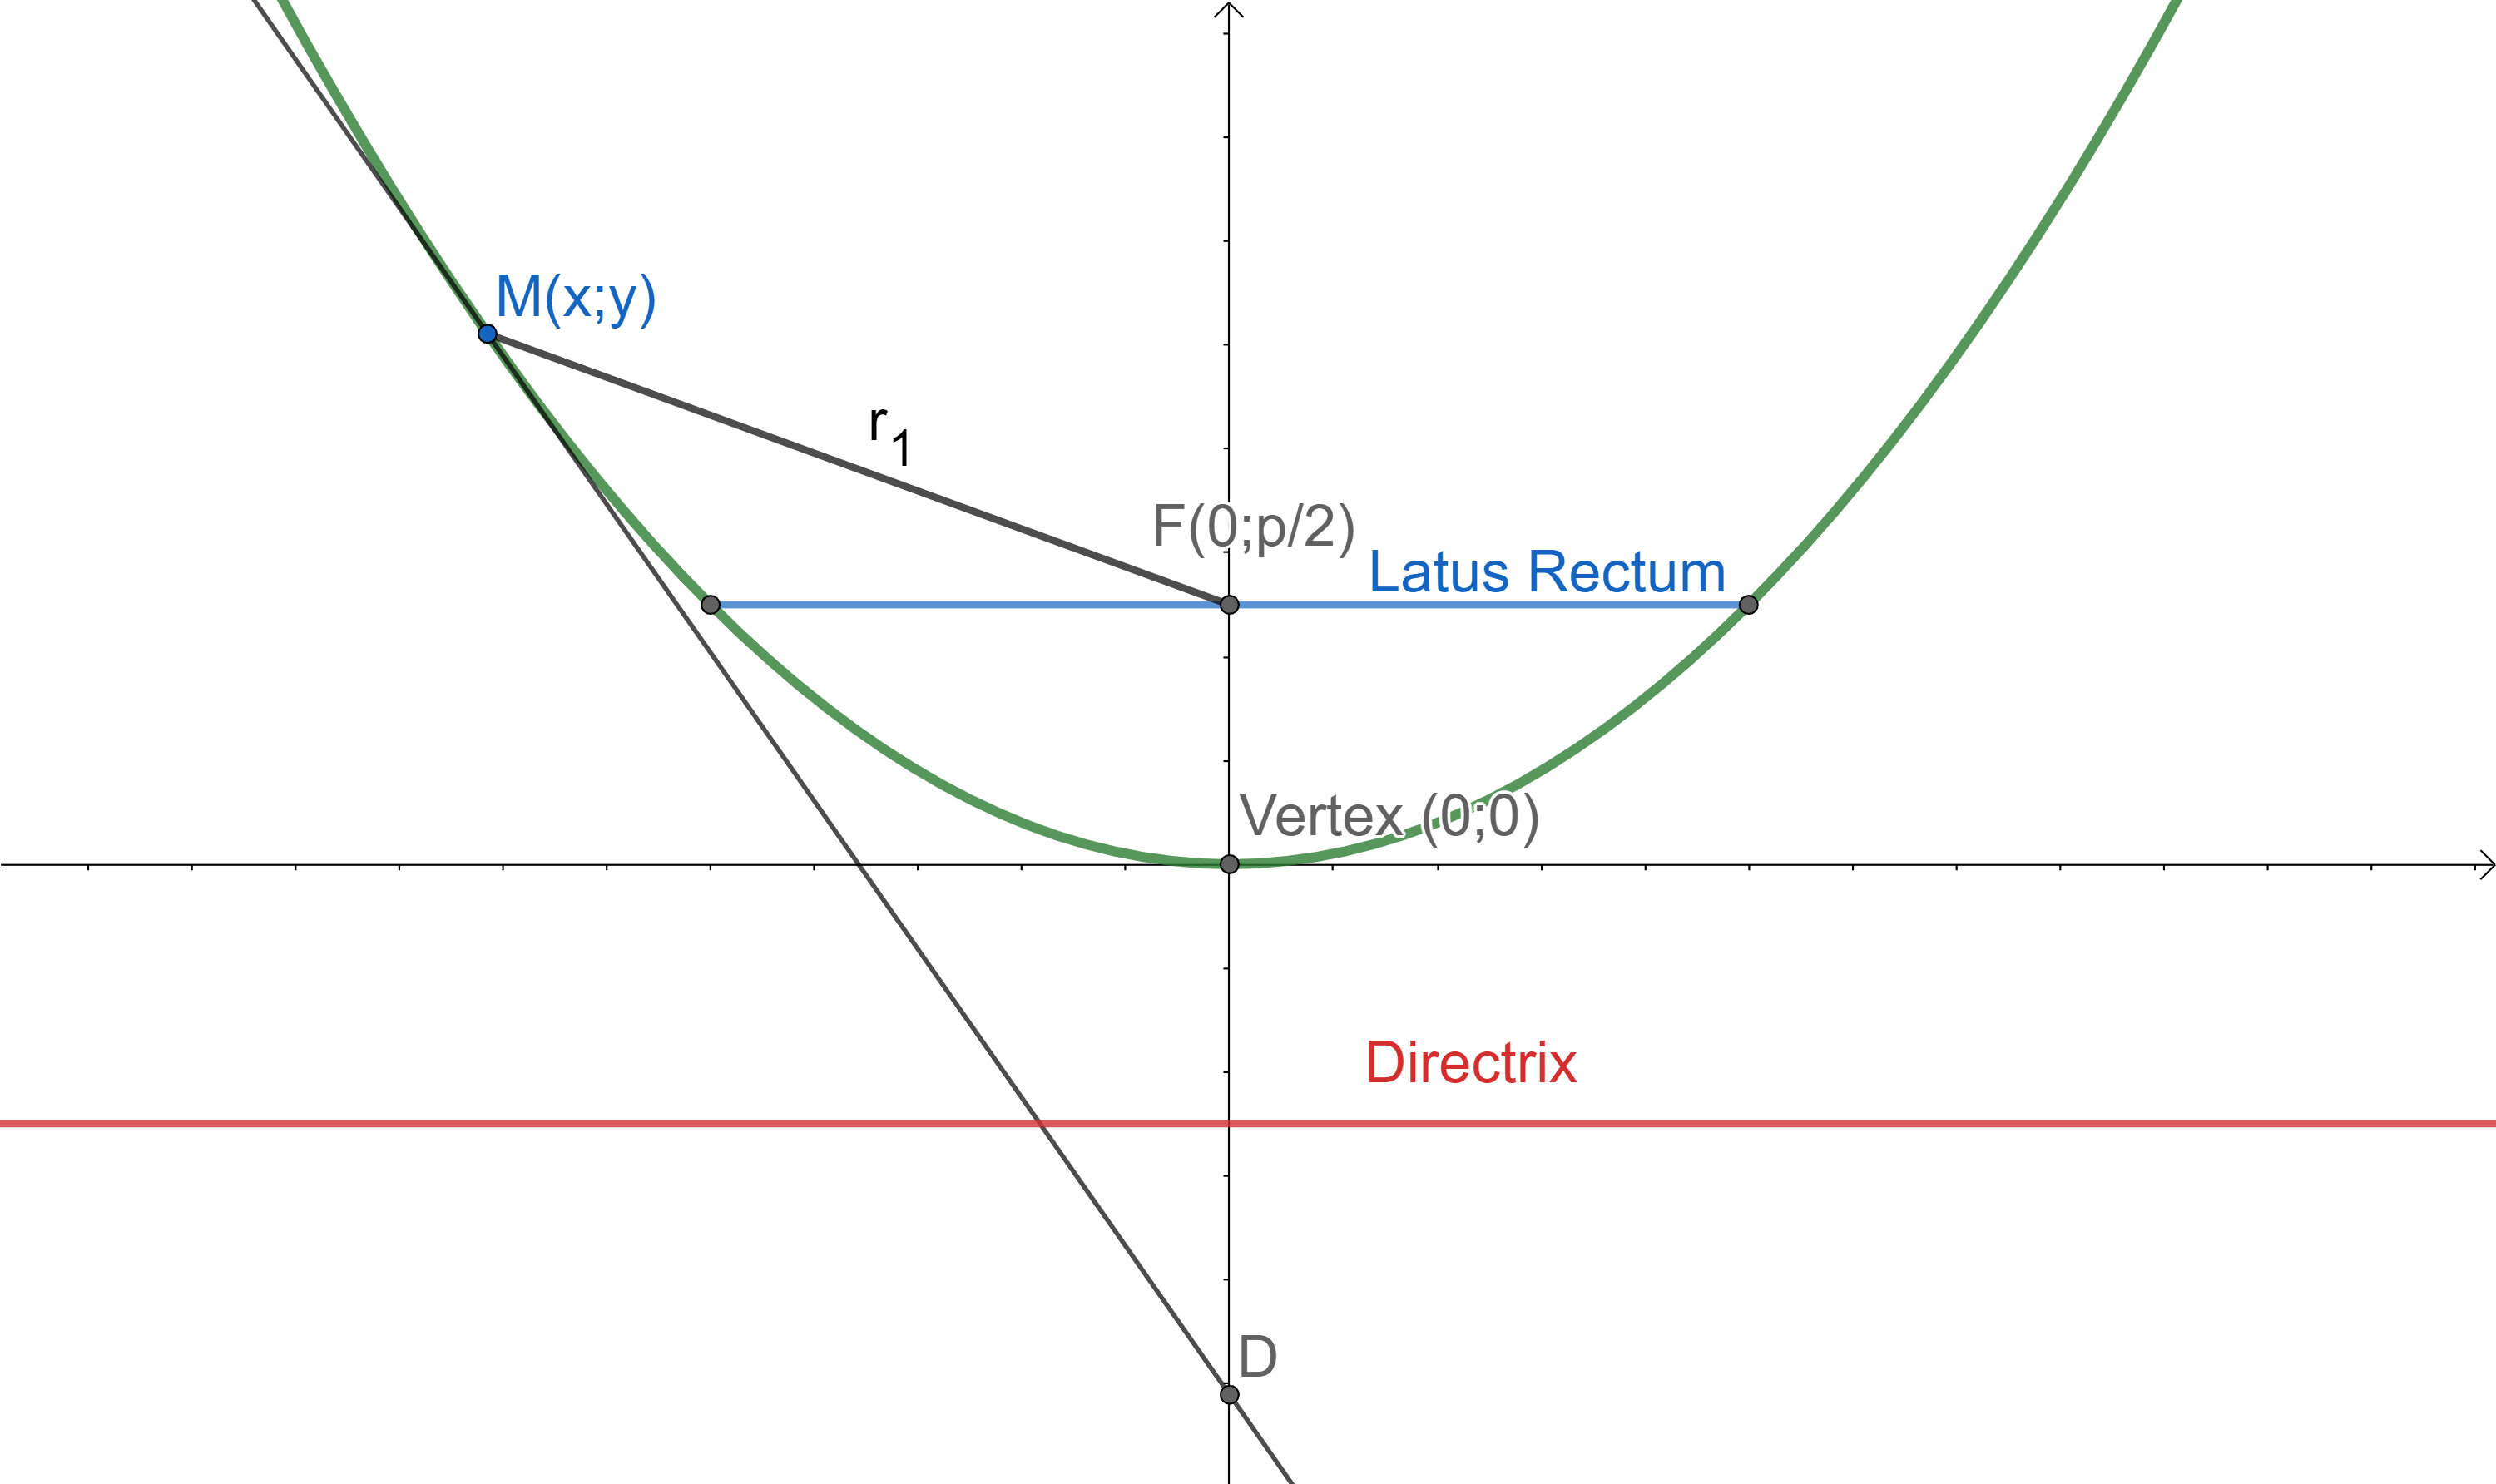
\includegraphics[height=3cm,width=1\textwidth,keepaspectratio]{Parabola.png}
            \vspace{-0.5cm}
            \caption*{\scriptsize Parabola $y=x^2$, $p=\dfrac{1}{2}$}
            \label{fig:Parabola.png}
        \end{figure}
    \end{column}
\end{columns}
\vspace{-0.6cm}
\textit{Properties:}
\begin{multicols}{3}
    \begin{itemize}
        \item \textbf{Vertex} $\begin{pmatrix} 0\\0 \end{pmatrix} + \begin{pmatrix} x_{\shf}\\y_{\shf} \end{pmatrix}$
        \item \textbf{Center} Not defined
        \item \textbf{Eccentricity} $e = 1$
        \item \textbf{Linear Eccentricity} Not defined
        \item \textbf{Foci} $F = \begin{pmatrix} 0\\\frac{p}{2} \end{pmatrix} + \begin{pmatrix} x_{\shf}\\y_{\shf} \end{pmatrix}$
        \item \textbf{Latus Rectum} (length of chord) $|2p|$
        \item \textbf{Focal parameter}  $p$
        \item \textbf{Discriminant} $\mathfrak{D} = B^2 - 4AC = 0$
        \item \textbf{Directrix eq.} $y = -\frac{p}{2} + y_{\shf}$
        \item \textbf{Tangent eq.}  $x(x_{\text{tan}}-x_{\shf})=p(y-y_{\text{tan}})+x_{\text{tan}}(x_{\text{tan}}-x_{\shf})$
        \item $r = |\overline{FM}|=\sqrt{(x-\frac{p}{2})^2+y^2}$
        \item $\triangle MFD$ is isosceles, where $MD$ -- tangent to $M$
        \end{itemize}
\end{multicols}
\end{frame}

\begin{frame}[t]{From general to canonical form}
\framesubtitle{When $B=0$}
    $Ax^2 +Cy^2 +2Dx + 2Ey +F = 0$ --- General form. \medskip

    Example of transformation from general to canonical form:
    \begin{align*}
        16x^2 + 25y^2 - 32x + 50y -359 = 0 \Rightarrow \\
        (16x^2 - 32x) + (25y^2 +50y) -359 = 0 \Rightarrow \\ 
        16(x^2 - 2x) + 25(y^2 + 2y) = 359 \Rightarrow \\ 
        16(x^2 -2x +1) + 25(y^2 +2y +1) = 350 + 16 + 25 \Rightarrow \\
        16(x-1)^2 +25(y+1)^2 = 400 \Rightarrow \\ 
        \frac{(x-1)^2}{25}+\frac{(y+1)^2}{16}=1
    \end{align*}
\end{frame}

\begin{frame}[t]{Task 1}
    \framesubtitle{}
    \only<1>{
        Find the foci, latus rectum, vertices and directrices of the following parabola: 
        $y^2+4x-2y+3=0$.}
    \only<2>{
        \alert{\Large Answer}
        \begin{figure}[H]
            \centering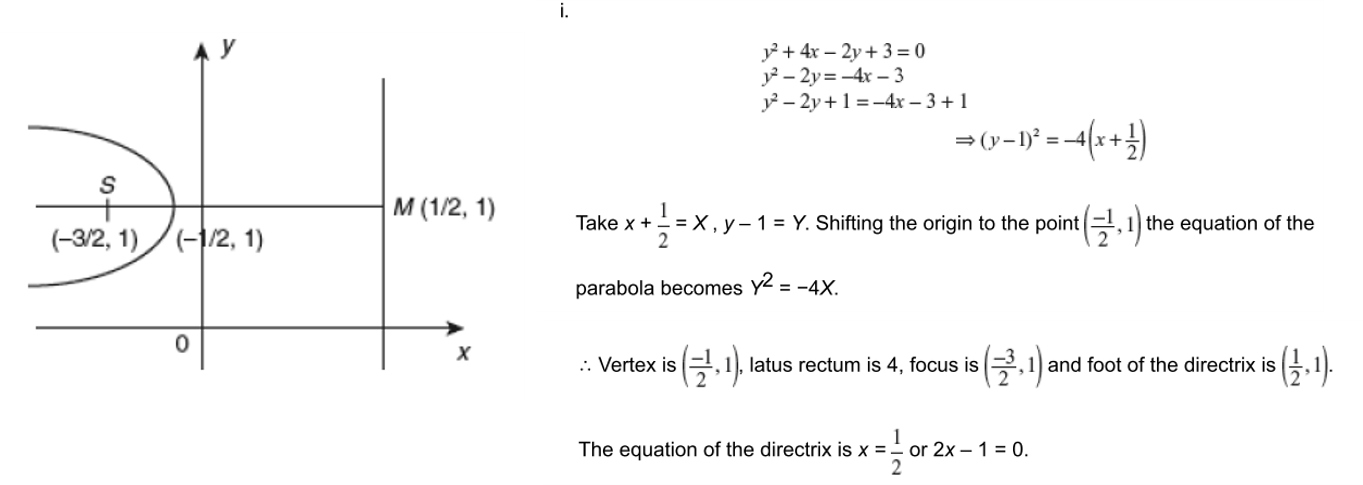
\includegraphics[height=5.5cm,width=1\textwidth,keepaspectratio]{1ans.png}
            % \caption{caption_name}
            \label{fig:1ans.png}
        \end{figure}
    }
\end{frame}
\begin{frame}[t]{Task 2}
    \framesubtitle{}
    \only<1>{
    Find the equations of the tangent and normal to the parabola $y^2 = 4(x-1)$ at $(5, 4)$.}
    \only<2>{
        \alert{\Large Answer}
        \vspace{-0.2cm}
        \begin{columns}[T,onlytextwidth]
            \begin{column}{0.64\textwidth}
                \begin{figure}[H]
                    \centering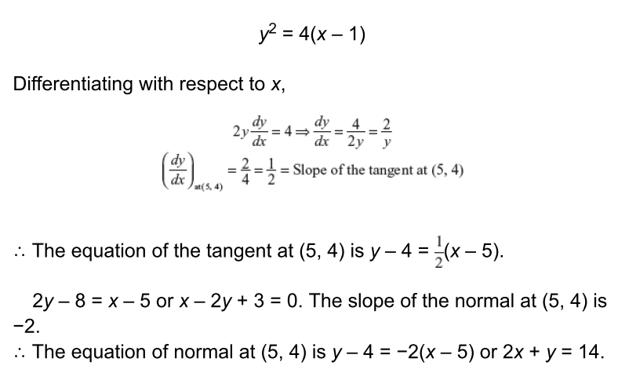
\includegraphics[height=5.5cm,width=1\textwidth,keepaspectratio]{2ans.png}
                    % \caption{caption_name}
                    \label{fig:2ans.png}
                \end{figure}
            \end{column}
            \begin{column}{0.34\textwidth}
                    \begin{figure}[H]
                        \href{https://www.geogebra.org/calculator/npd7exdq}{
                            \centering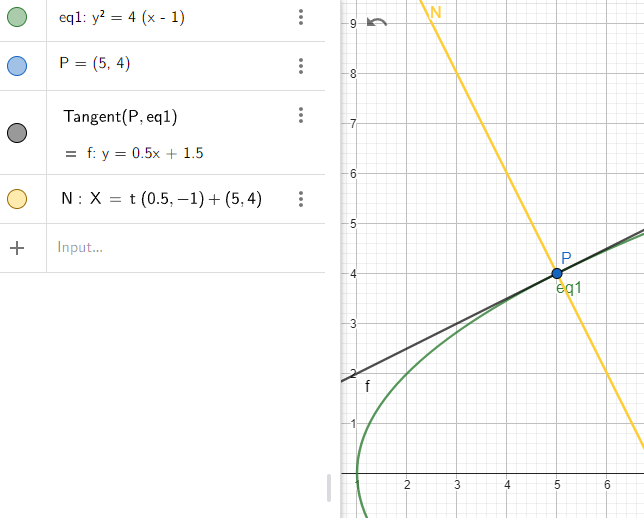
\includegraphics[height=5cm,width=1\textwidth,keepaspectratio]{2ans_1.png}}
                        \label{fig:2ans_1.png}
                    \end{figure}
            \end{column}
        \end{columns}
    }
\end{frame}

\begin{frame}[t]{Task 3}
    \framesubtitle{}
    \only<1>{
        An equilateral triangle is inscribed in the parabola $y^2 = 4ax$ one of whose vertices is at the vertex of the parabola. Find its side.}
    \only<2>{
        \alert{\Large Answer}
        \begin{figure}[H]
            \centering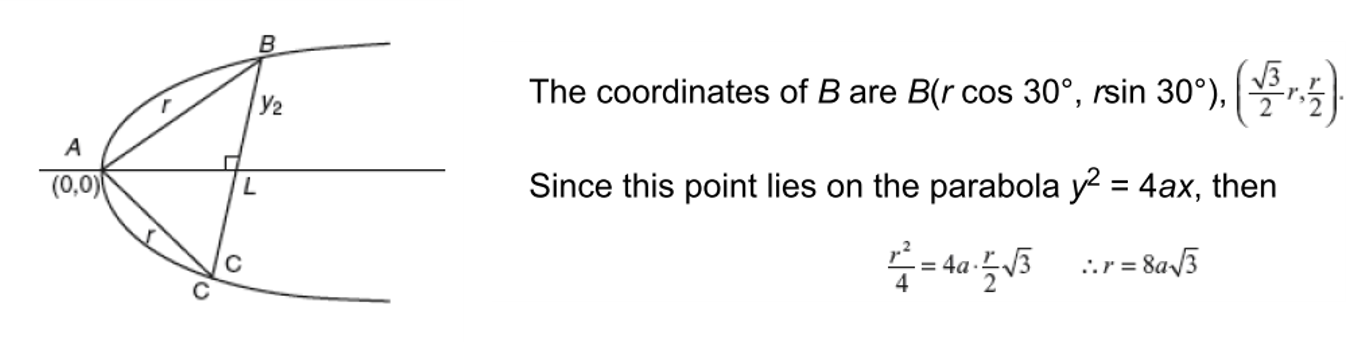
\includegraphics[height=5.5cm,width=1\textwidth,keepaspectratio]{3ans.png}
            % \caption{caption_name}
            \label{fig:3ans.png}
        \end{figure}
    }
\end{frame}

\begin{frame}[t]{Task 4}
    \framesubtitle{}
    \only<1>{
        Find the equation of a parabola that has a line $x=8$ for a directrix and point $F(7;0)$ for a focus.
    }
    \only<2>{
        \alert{\Large Answer}
        \begin{figure}[H]
            \centering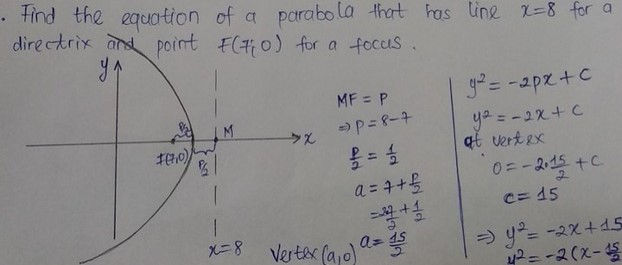
\includegraphics[height=5.5cm,width=1\textwidth,keepaspectratio]{4ans.jpg}
            % \caption{caption_name}
            \label{fig:4ans.jpg}
        \end{figure}
    }
\end{frame}

\begin{frame}[t]{Collisions}
    \framesubtitle{Video}
    \vspace{-0.6cm}
    \begin{figure}[H]
        \href{https://youtu.be/aTbw71EpamY}{
            \centering
\includegraphics[height=6cm,width=1\textwidth,keepaspectratio]{collisions.jpg}}
        % \caption{Click on a picture for a video}
        \label{fig:collisions.jpg}
    \end{figure}
\end{frame}

\begin{frame}[t]{Ellipse}
    \framesubtitle{}
        \scriptsize
        \vspace{-0.4cm}
    \begin{columns}[T,onlytextwidth]
        \begin{column}{0.59\textwidth}
            \textit{Forms:} \\
            \begin{itemize}
                \item \textbf{Canonical} $\frac{(x-x_{\shf})^2}{a^2}+\frac{(y-y_{\shf})^2}{b^2}=1$
                \item \textbf{General} $Ax^2+Bxy+Cy^2+Dx+Ey+F=0$, where $AC > 0$, if $B=0$
                \item \textbf{Parametric} $\left\{\begin{matrix*}[l] x = a\cos(\alpha)\\ y = b\sin(\alpha) \end{matrix*}\right.$
            \end{itemize}
        \end{column}
        \begin{column}{0.39\textwidth}
            \vspace{-0.5cm}
            \begin{figure}[H]
                \centering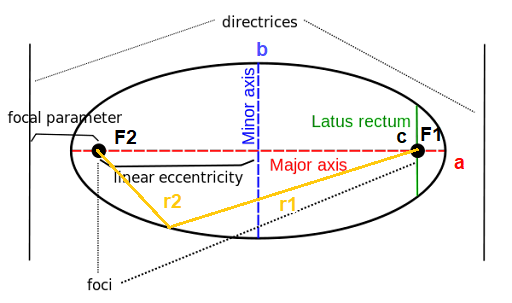
\includegraphics[height=3cm,width=1\textwidth,keepaspectratio]{Ellipse.png}
                \vspace{-0.5cm}
                \caption*{\scriptsize Ellipse $\frac{x^2}{a^2}+\frac{y^2}{b^2}=1$}
                \label{fig:Ellipse.png}
            \end{figure}
        \end{column}
    \end{columns}
    \vspace{-0.5cm}
    \textit{Properties:}
    \vspace{-0.2cm}
    \begin{multicols}{3}
        \begin{itemize}
            \item \textbf{Vert} $\begin{pmatrix} \pm a\\0 \end{pmatrix}$\&$\begin{pmatrix} 0\\\pm b \end{pmatrix}$ $ + \begin{pmatrix} x_{\shf}\\y_{\shf} \end{pmatrix}$
            \item \textbf{Center} $(0;0) + (x_{\shf};y_{\shf})$
            \item \textbf{Eccentricity} $0 \leq e < 1$, $e = \sqrt{1 - \frac{b^2}{a^2}}$
            \item \textbf{Linear Eccentricity} $c = \sqrt{a^2-b^2}$
            \item \textbf{Foci} $F = \begin{pmatrix} \pm(c= e\ a)\\ 0 \end{pmatrix} + \begin{pmatrix} x_{\shf}\\y_{\shf} \end{pmatrix}$
            \item \textbf{Latus Rectum} (length of chord) $\frac{2b^2}{a}$
            \item \textbf{Focal parameter}  $\frac{b^2}{\sqrt{a^2-b^2}}$
            \item \textbf{Discriminant} $\mathfrak{D} = B^2 - 4AC < 0$
            \item \textbf{Directrix eq.} $x = \pm \frac{a}{e} + x_{\shf}$
            \item \textbf{Tangent eq. (w/o shift)} $\dfrac{x_{tangent} x}{a^2}+\dfrac{y_{tangent} y}{b^2}=1$
            \item $r_1 + r_2 = 2a$
            \item $r_{1,2} = |\overline{F_{1,2}M}|=\sqrt{(x \pm c)^2+y^2}$
            \item $\frac{r_1}{d_1}=e$
            \end{itemize}
    \end{multicols}
    \end{frame}

    \begin{frame}[t]{Task 5}
        \framesubtitle{}
        \only<1>{
            Find the equation of the ellipse whose foci are $(4, 0)$ and $(-4, 0)$ and $e=1/3$}
        \only<2>{
            \alert{\Large Answer}
            \begin{figure}[H]
                \centering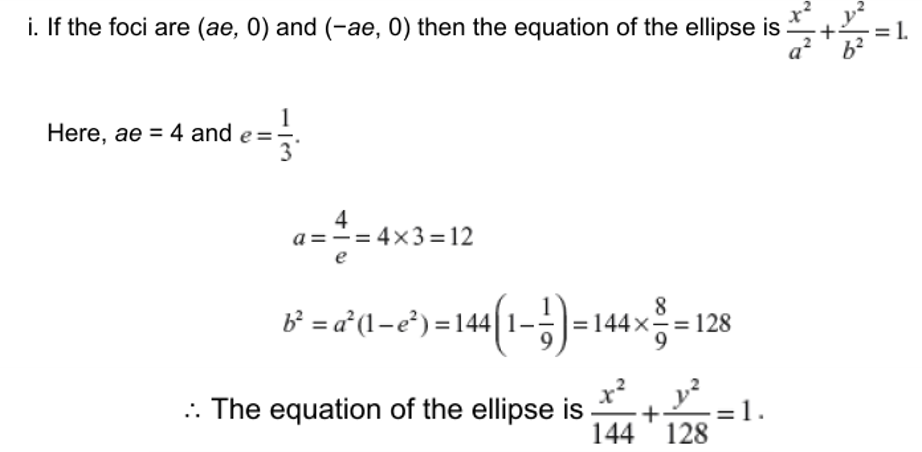
\includegraphics[height=5.5cm,width=1\textwidth,keepaspectratio]{5ans.png}
                % \caption{caption_name}
                \label{fig:5ans.png}
            \end{figure}
        }
    \end{frame}

    \begin{frame}[t]{Task 6}
        \framesubtitle{}
        \only<1>{
            Find the eccentricity, foci and the length of the latus rectum of the ellipse 
            $9x^2+4y^2=36$}
        \only<2>{
            \alert{\Large Answer}
            \begin{figure}[H]
                \centering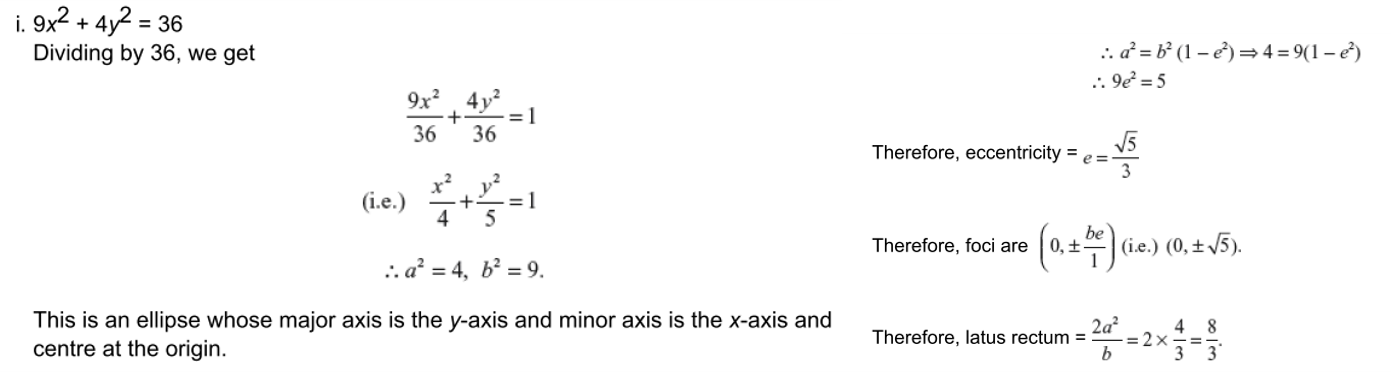
\includegraphics[height=5.5cm,width=1\textwidth,keepaspectratio]{6ans.png}
                % \caption{caption_name}
                \label{fig:6ans.png}
            \end{figure}
        }
    \end{frame}

    \begin{frame}[t]{Task 7}
        \framesubtitle{}
        \only<1>{
            The equation $25(x^2 - 6x + 9) + 16y^2 = 400$ represents an ellipse. Find the centre and foci of the ellipse. How should the axis be transformed so that the ellipse is represented by the equation  $\dfrac{x^2}{25}+\dfrac{y^2}{16} = 1$?}
        \only<2>{
            \alert{\Large Answer}
            \begin{figure}[H]
                \centering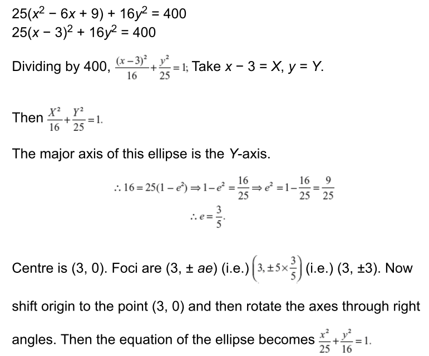
\includegraphics[height=5.5cm,width=1\textwidth,keepaspectratio]{7ans.png}
                % \caption{caption_name}
                \label{fig:7ans.png}
            \end{figure}
        }
    \end{frame}

    \begin{frame}[t]{Task 8}
        \framesubtitle{}
        \only<1>{
            Find the eccentricity of an ellipse given that:
            \begin{enumerate}
                \item its major axis subtends an angle of $120^\circ$ at the endpoints of its minor axis;
                \item the segment between a focus and the farthest vertex subtends an angle of $90^{\circ}$ at the endpoints of its minor axis.
            \end{enumerate}
        }
        \only<2>{
            \alert{\Large Answer}
            \begin{figure}[H]
                \centering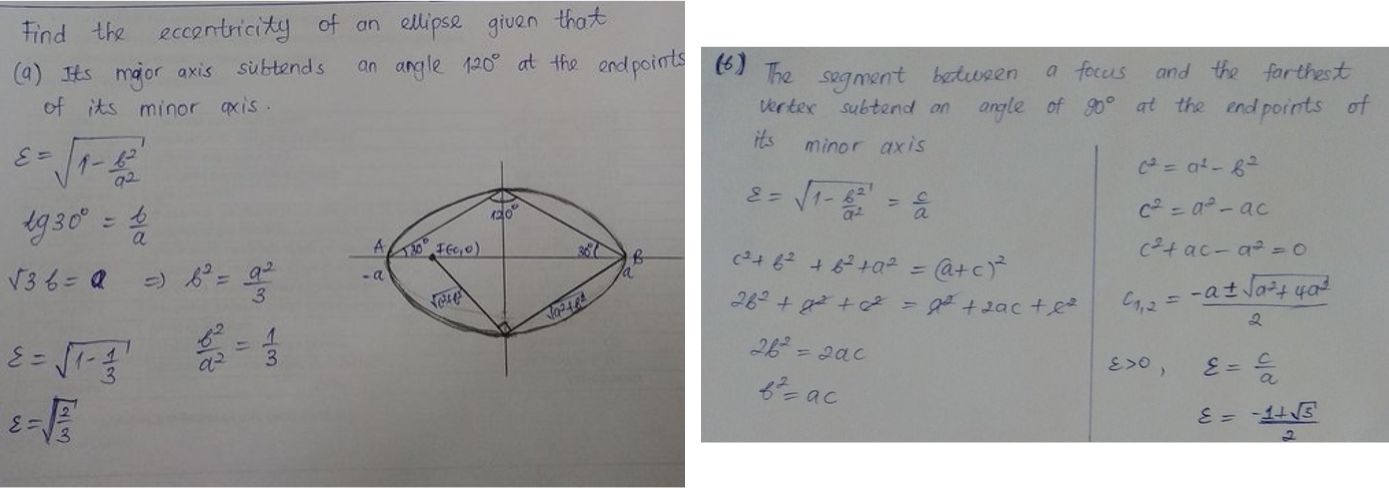
\includegraphics[height=5.5cm,width=1\textwidth,keepaspectratio]{8ans.png}
                % \caption{caption_name}
                \label{fig:8ans.png}
            \end{figure}
        }
    \end{frame}


\begin{frame}[t]{Reference material}
    % \framesubtitle{OnlineMschool}
    \Large
    \begin{itemize}
        \item \href{https://en.wikipedia.org/wiki/Conic_section}{Conics Section (Wiki)}
        \item \href{https://www.youtube.com/playlist?list=PLXSlB4yMaoJsSuwwC1TaR7mATy2ZARHvi}{Conic sections (Khan Academy, full playlist, eng)}
    \end{itemize}
\end{frame}

\fbckg{fibeamer/figs/last_page.png}
\frame[plain]{}

\end{document}